\begin{table}[t]
\centering
\caption{Held-out FS2K test results for the selected local conditional GAN (1,046 paired images). The style-macro row weights each style equally.}
\label{tab:fs2k}
\begin{tabular}{lrrrr}
\toprule
Style & $n$ & MAE $\downarrow$ & SSIM $\uparrow$ & PSNR $\uparrow$ \\
\midrule
1 & 619 & 0.0871 & 0.4982 & 16.57 \\
2 & 381 & 0.1662 & 0.3594 & 11.67 \\
3 & 46 & 0.0724 & 0.5724 & 17.73 \\
\midrule
Overall & 1,046 & 0.1153 & 0.4509 & 14.83 \\
Style macro & -- & 0.1085 & 0.4767 & 15.32 \\
\bottomrule
\end{tabular}
\end{table}

The FS2K model was selected by validation and evaluated once on the held-out test split. Style 2 has the largest reconstruction error, while style 3 has the lowest. These scores measure similarity to the annotated paired sketch, not artistic preference. Figure~\ref{fig:fs2k-samples} shows examples across all three styles, and Figure~\ref{fig:fs2k-failures} shows the lowest-SSIM test cases.

\begin{figure}[t]
\centering
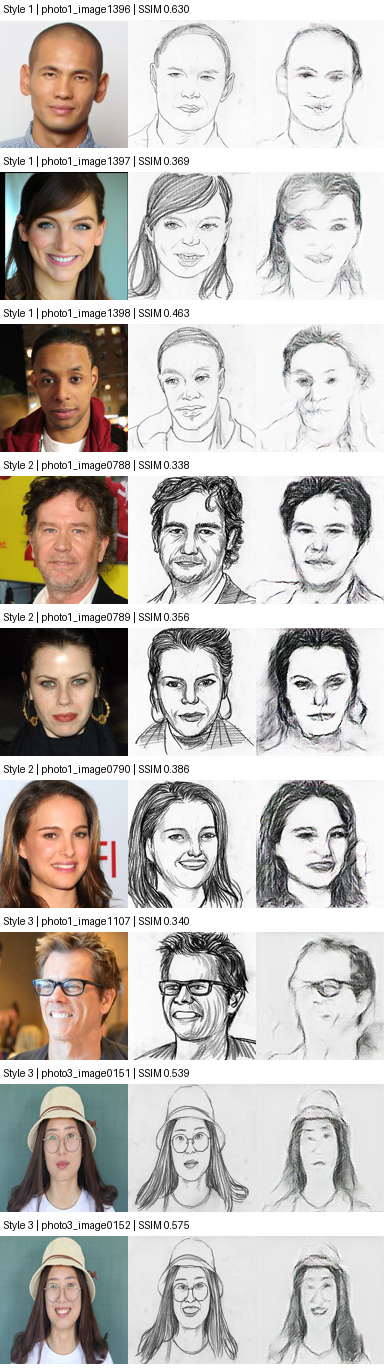
\includegraphics[width=\columnwidth]{figures/task4_samples.png}
\caption{FS2K test examples: input photograph, paired target, generated sketch.}
\label{fig:fs2k-samples}
\end{figure}

\begin{figure}[t]
\centering
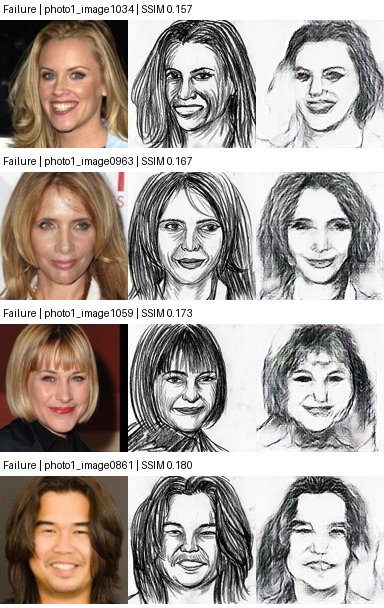
\includegraphics[width=\columnwidth]{figures/task4_failures.png}
\caption{Four held-out FS2K cases with the lowest structural similarity.}
\label{fig:fs2k-failures}
\end{figure}

\begin{table}[t]
\centering
\caption{Task 1 universal autoencoder on the untouched Oxford-IIIT Pet test set. Each row contains 3,669 images.}
\label{tab:task1}
\begin{tabular}{llrrr}
\toprule
Condition & Severity & MAE $\downarrow$ & SSIM $\uparrow$ & PSNR $\uparrow$ \\
\midrule
Clean & none & 0.0355 & 0.8068 & 25.84 \\
Salt-and-pepper & low & 0.0355 & 0.8006 & 25.88 \\
Salt-and-pepper & medium & 0.0363 & 0.7873 & 25.74 \\
Salt-and-pepper & high & 0.0390 & 0.7602 & 25.21 \\
Gaussian blur & low & 0.0345 & 0.8088 & 26.16 \\
Gaussian blur & medium & 0.0347 & 0.7888 & 26.11 \\
Gaussian blur & high & 0.0400 & 0.7174 & 24.80 \\
Occlusion & low & 0.0420 & 0.7595 & 23.64 \\
Occlusion & medium & 0.0486 & 0.7132 & 22.15 \\
Occlusion & high & 0.0599 & 0.6414 & 20.37 \\
\bottomrule
\end{tabular}
\end{table}

The selected Task 1 configuration used learning rate $1.03\times10^{-4}$, batch size 16, 24 base channels, a 48-channel bottleneck, and $\alpha=0.526$. The bounded search completed three trials; the selected trial's short-run validation objective was 0.1421. A matched four-epoch follow-up varied only autoencoder dropout: 0.0 achieved validation objective 0.1438 versus 0.1488 at dropout 0.2, on the same 128 validation IDs and 75 training steps per epoch. This short comparison favors no dropout but does not prove the ranking would persist over a full training run. Final training reached epoch 35, with best full-validation objective 0.07750 at epoch 33. On the 36,690 fixed test cases, high occlusion is the most difficult condition (MAE 0.0599, SSIM 0.6414), while low blur is the strongest (MAE 0.0345, SSIM 0.8088). This gap is consistent with the information loss from large masked regions; the remaining errors are visible in the example and failure panels.

\begin{figure}[t]
\centering
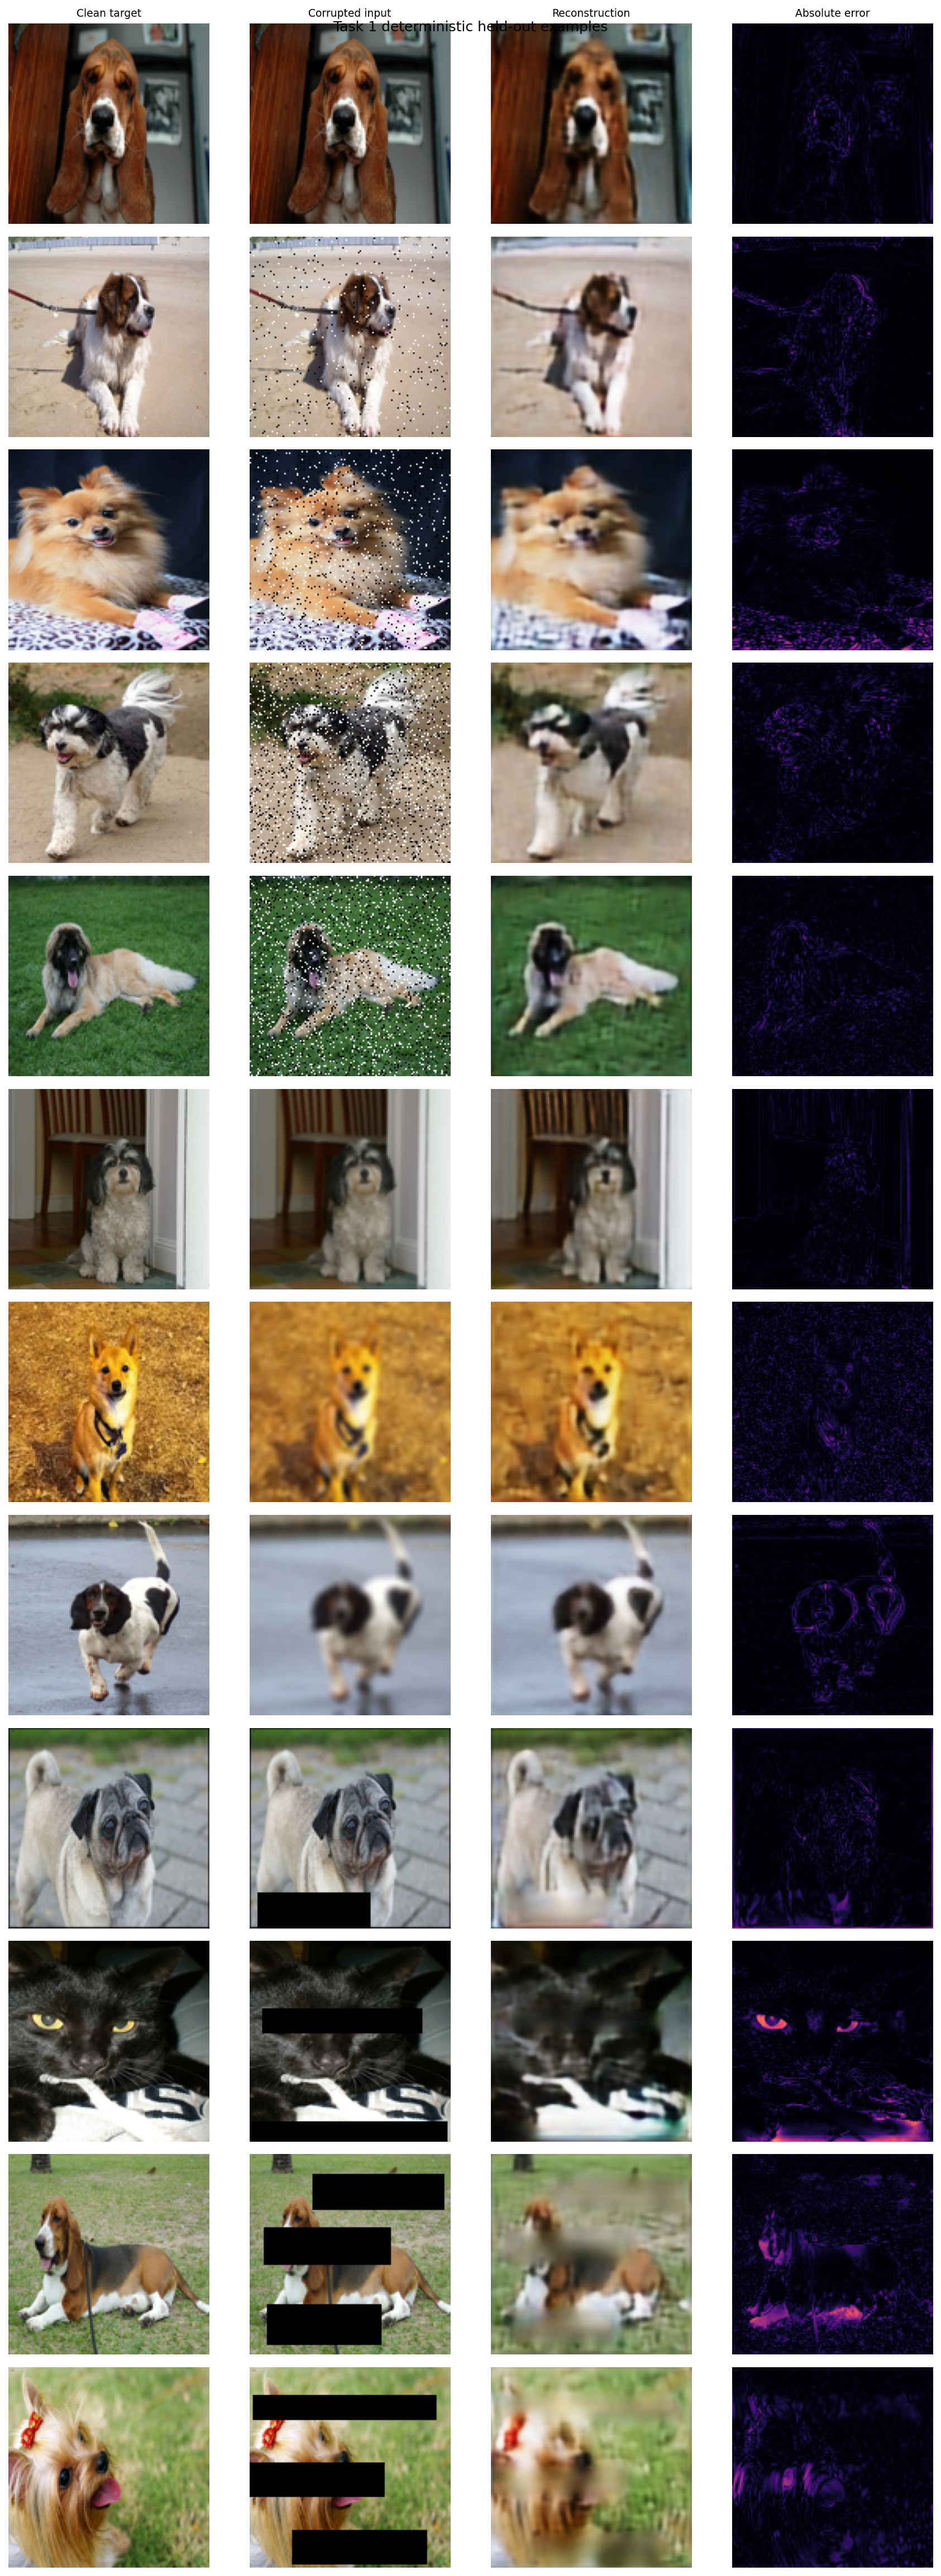
\includegraphics[width=\columnwidth]{figures/task1_examples.png}
\caption{Twelve Task 1 test cases with clean target, corrupted input, reconstruction, and absolute error map.}
\label{fig:task1-examples}
\end{figure}

\begin{figure}[t]
\centering
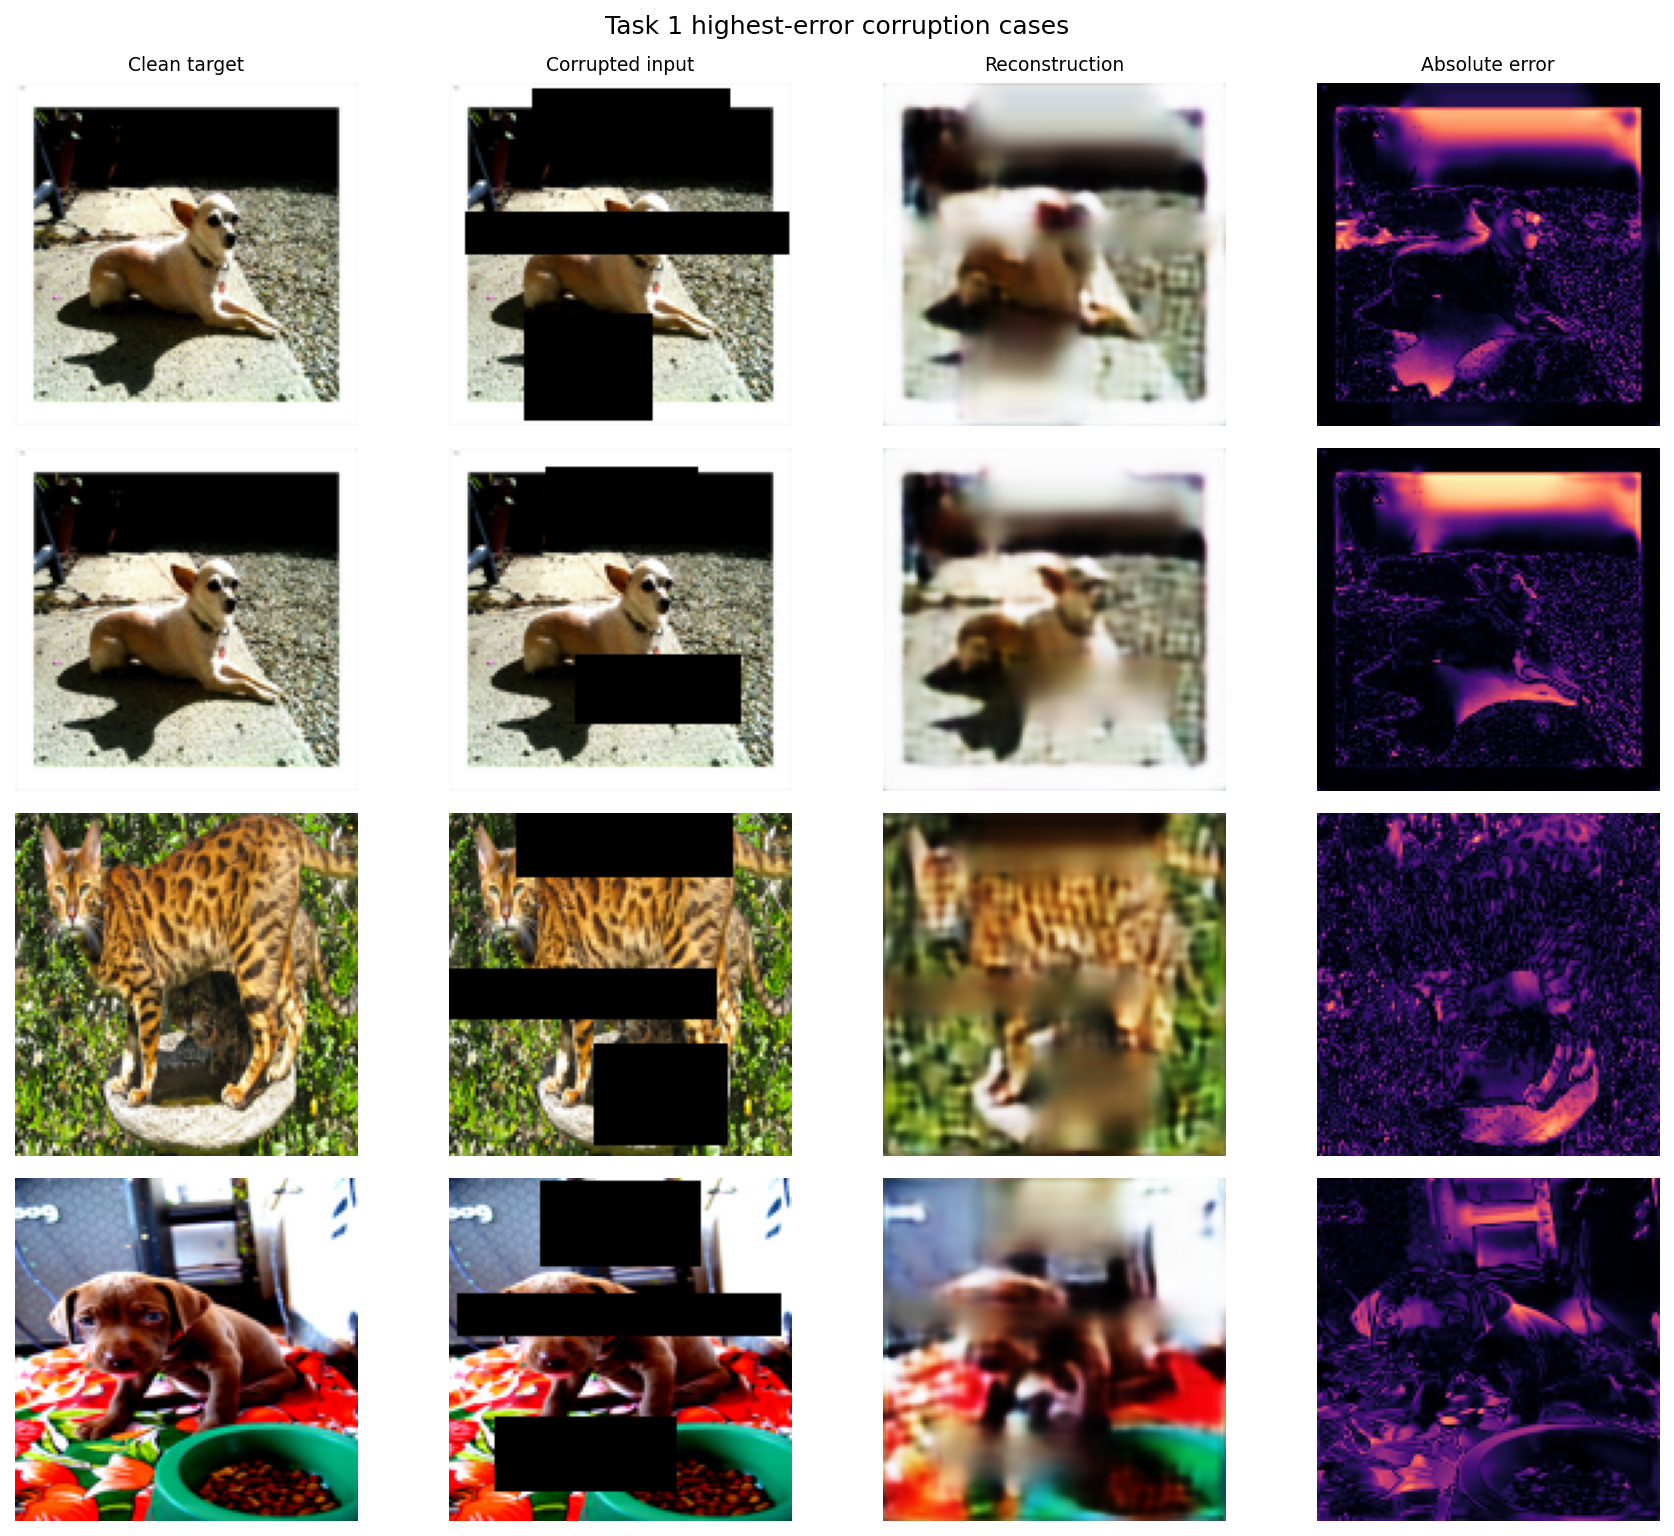
\includegraphics[width=\columnwidth]{figures/task1_failures.png}
\caption{Four highest-error Task 1 test cases selected from the fixed corruption manifest.}
\label{fig:task1-failures}
\end{figure}

Task 2's selected classifier checkpoint (epoch 22) was assessed on the 7,360 deterministic validation cases. It reached 99.58\% accuracy and 0.9931 macro-F1. The remaining errors are concentrated in clean-versus-blur and occlusion-versus-clean confusions; the specialist routing results are reported separately after expert training.

\begin{table}[t]
\centering
\caption{Task 2 classifier validation results.}
\label{tab:classifier-validation}
\begin{tabular}{lrrrr}
\toprule
Class & Support & Precision & Recall & F1 \\
\midrule
Clean & 736 & 0.9719 & 0.9878 & 0.9798 \\
Salt-and-pepper & 2,208 & 0.9991 & 1.0000 & 0.9995 \\
Gaussian blur & 2,208 & 0.9986 & 0.9973 & 0.9980 \\
Occlusion & 2,208 & 0.9977 & 0.9928 & 0.9952 \\
\midrule
Macro average & 7,360 & 0.9918 & 0.9945 & 0.9931 \\
\bottomrule
\end{tabular}
\end{table}

\begin{figure}[t]
\centering
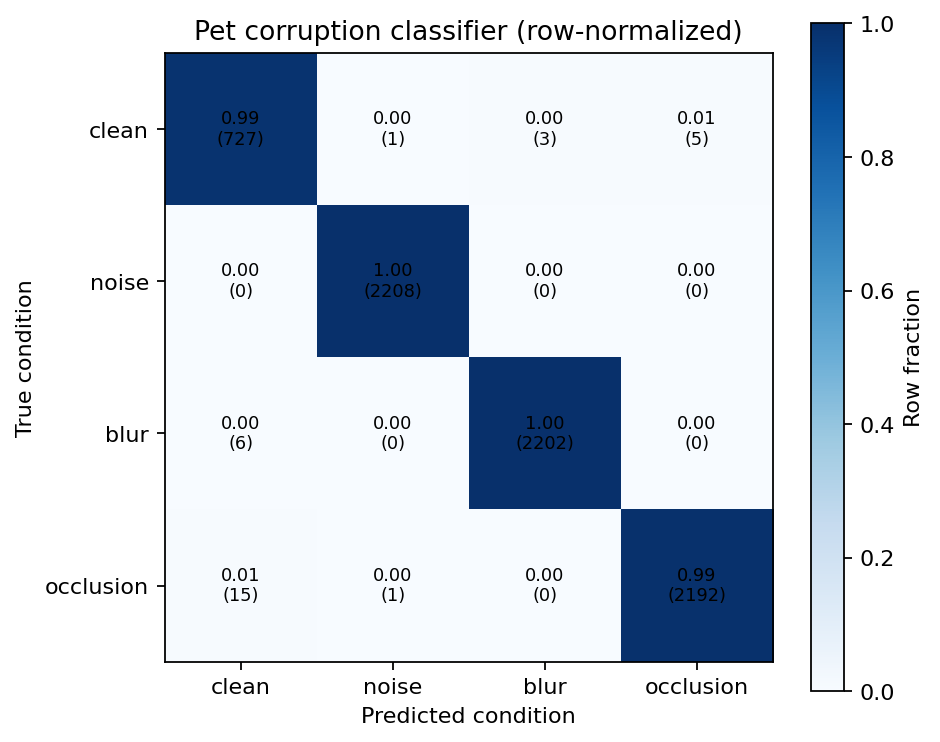
\includegraphics[width=0.76\columnwidth]{figures/task2_classifier_confusion.png}
\caption{Task 2 corruption classifier row-normalized validation confusion matrix; counts are annotated in parentheses.}
\label{fig:task2-classifier-confusion}
\end{figure}
